\documentclass{article}
\usepackage[utf8]{inputenc}
\usepackage[spanish]{babel}
\usepackage{listingsutf8}
\usepackage{xcolor}
\usepackage{pdfpages}
\usepackage{geometry}
% to install algorithm2e pckg: sudo apt-get install texlive-science
\usepackage[ruled, vlined, nofillcomment]{algorithm2e}

\geometry{
    a4paper,
    margin=1.2in
}

\title{75.29 - Teoría de Algoritmos I: Trabajo Práctico n. 2}
\author{
    \\\\\\\\
    \Large{Equipo Q:}\\
    Lavandeira, Lucas (\texttt{\#98042})\\\texttt{}\\
    \\
    Rozanec, Matias (\texttt{\#97404})\\\texttt{rozanecm@gmail.com}\\
    \\
    Sbruzzi, José (\texttt{\#97452})\\\texttt{}\\
    \\\\\\\\\\\\\\
}
\date{14.mayo.2018}

\begin{document}
\maketitle
\begin{figure}[!htp]
    \centering
    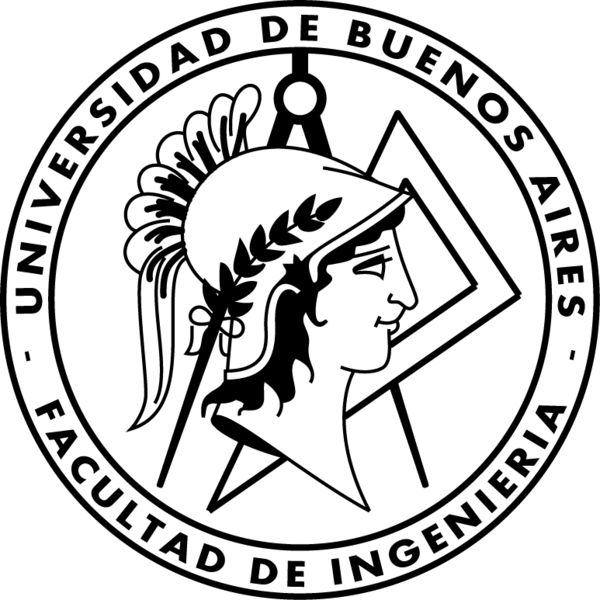
\includegraphics[scale=1]{res/fiuba_logo.png} 
\end{figure}
\begin{center}\normalsize{Facultad de Ingeniería, Universidad de Buenos Aires}\end{center}
\newpage

\tableofcontents
\newpage

% *** RESOLUCION ***
% Some settings for coding style
\lstset{
    basicstyle=\linespread{0.9}\ttfamily\footnotesize,
    frame=single,
    frameround=tttt,
    numbers=left,
    numberstyle=\tiny,
    linewidth=14cm,
    literate=
      {á}{{\'a}}1 {é}{{\'e}}1 {í}{{\'i}}1 {ó}{{\'o}}1 {ú}{{\'u}}1
      {Á}{{\'A}}1 {É}{{\'E}}1 {Í}{{\'I}}1 {Ó}{{\'O}}1 {Ú}{{\'U}}1
      {à}{{\`a}}1 {è}{{\`e}}1 {ì}{{\`i}}1 {ò}{{\`o}}1 {ù}{{\`u}}1
      {À}{{\`A}}1 {È}{{\'E}}1 {Ì}{{\`I}}1 {Ò}{{\`O}}1 {Ù}{{\`U}}1
      {ä}{{\"a}}1 {ë}{{\"e}}1 {ï}{{\"i}}1 {ö}{{\"o}}1 {ü}{{\"u}}1
      {Ä}{{\"A}}1 {Ë}{{\"E}}1 {Ï}{{\"I}}1 {Ö}{{\"O}}1 {Ü}{{\"U}}1
      {â}{{\^a}}1 {ê}{{\^e}}1 {î}{{\^i}}1 {ô}{{\^o}}1 {û}{{\^u}}1
      {Â}{{\^A}}1 {Ê}{{\^E}}1 {Î}{{\^I}}1 {Ô}{{\^O}}1 {Û}{{\^U}}1
      {œ}{{\oe}}1 {Œ}{{\OE}}1 {æ}{{\ae}}1 {Æ}{{\AE}}1 {ß}{{\ss}}1
      {ű}{{\H{u}}}1 {Ű}{{\H{U}}}1 {ő}{{\H{o}}}1 {Ő}{{\H{O}}}1
      {ç}{{\c c}}1 {Ç}{{\c C}}1 {ø}{{\o}}1 {å}{{\r a}}1 {Å}{{\r A}}1
      {€}{{\euro}}1 {£}{{\pounds}}1 {«}{{\guillemotleft}}1
      {»}{{\guillemotright}}1 {ñ}{{\~n}}1 {Ñ}{{\~N}}1 {¿}{{?`}}1
}
\part{Resolución}
\section{Parte 1: Spy vs Spy}

\subsection{Caminos sin costos}
Para resolver el problema partimos de la idea de que el espía que está mas cerca del aeropuerto se queda con los documentos. Así, para resolver el problema con costos unitarios, sedecidió hacer una versión modificada de BFS, partiendo desde el aeropuerto. Así, el algoritmo a medida que se ejecuta descubre "capas" en el grafo, donde cada capa está a una distancia mayor del aeropuerto que la anterior. El algoritmo se detiene cuando descubre una capa que contiene al menos un espía. De esta forma determina el más cercano, o indica que ambos están a la misma distancia.

[[poner un dibujito acáaaa]]

\subsubsection{Complejidad del algoritmo para caminos sin costos}

En el archivo \texttt{problema.clj} se abstrajo lo que tienen en común las dos situaciones a resolver: que la solución se realiza con la estrategia greedy. Así, \texttt{solucion-greedy} se llamará una vez para cada una delas alternativas que surjan. Debido a la naturaleza de Breadth-First-Search (\texttt{bfs.clj}), podemos determinar que esta función se ejecutará, como mucho, una vez por cada vértice.

Los pasos \texttt{terminado?}, \texttt{conclusion} son \textit{O(1)} si se considera que el tamaño de la lista \texttt{hasta} es constante, lo cual es verdadero para el problema en cuestión. Se utilizan los conjuntos y diccionarios del lenguaje para brindar acceso en tiempo constante. Sin embargo, la función \texttt{alternativa} tiene una duración que crece linealmente con la cantidad de \texttt{vecinos} que tenga el vértice \texttt{actual}. Si \texttt{alternativa} se ejecuta para todos los vértices del grafo, la cantidad acumulada de vecinos será el doble de la cantidad de aristas del grafo. Así, el algoritmo implementado tiene una complejidad temporal igual a la de BFS: \textit{O(|V|+|E|)}.

Agregando la etapa en que se retorna el camino recorrido por cada espia, la complejidad sólo puede llegar a \textit{O(|V|)}, ya que durante el algoritmo se calculan todas las distancias necesarias para alcanzar los espías desde el aeropuerto: El algoritmo que forma este camino sólo tiene que recorrer el grafo desde los puntos de partida de cada espía eligiendo como siguiente nodo el vecino con menor distancia al aeropuerto.

Por lo tanto, incorporando esta etapa, la complejidad temporal sigue siendo \textit{O(|V|+|E|)}.

\subsection{}



\section{Parte 2}
\subsection{Ejercicio 1}
El problema a resolver es uno de detección de rotaciones cíclicas en dos strings (cadenas de caracteres). Un string es una rotación cíclica de otro cuando, al ``conectar" el principio y el fin de cada una, se tenga como resultado ciclos indistinguibles uno del otro. Por ejemplo, el \texttt{ABCD} y \texttt{CDAB} son rotaciones cíclicas uno del otro, porque los ciclos \texttt{ABCDABCDABCD...} y \texttt{CDABCDABCDAB...} son indistinguibles si no sabemos su punto de inicio. El problema puede ser caracterizado como uno de decisión, simplemente queremos saber si se cumple la condición pedida o no, es decir, los algoritmos a implementar simplemente devuelven un valor booleano, verdadero o falso. Se pide resolverlo usando distintos algoritmos y comparar sus órdenes de tiempo de ejecución.

La primera solución a implementar es por fuerza bruta. Si asumimos que la comparación de strings es de orden lineal, ir haciendo la rotación de uno de los dos strings y comparando hasta llegar a una igualdad da como resultado un algoritmo de orden cuadrático en el peor caso, cuando se prueban todas las rotaciones y la última (o ninguna) comparación da verdadera.

La segunda solución es implementando el algoritmo KMP de \textit{string matching}. El algoritmo se puede resumir en una forma optimizada de decidir si una palabra \textit{word} está contenida dentro de un texto fuente \textit{text} en orden lineal, realizando un precómputo de una tabla de valores que asisten al algoritmo durante la ejecución. El caso de uso común de KMP es para ubicar una única palabra en un texto grande, mientras que nuestro problema es diferente, queremos decir si un string es una rotación cíclica de otro. Lo que hacemos es ejecutar el algoritmo bajo un ciclo \textit{for}, rotando uno de los strings entre cada iteración. El algoritmo KMP es de orden lineal de la longitud del texto, que para nuestro caso es el mismo que el de la palabra.

Esta aplicación se puede ver como una \textit{reducción} de un problema a otro. Las reducciones son una herramienta que nos permite obtener información de la complejidad de un algoritmo desconocido, basándonos en uno conocido. Llamemos al algoritmo que no conocemos como X, y al que sí, como Y. Si podemos resolver X utilizando a un algoritmo que resuelve Y como una caja negra, utilizándola una cantidad polinomial de veces, se pueden establecer relaciones entre las complejidades de ambos problemas.

En particular, la reducción que nos interesa es X siendo el problema de rotaciones cíclicas, Y el de string matching, y nuestra caja negra es el algoritmo KMP. Al ejecutar el algoritmo unas N veces en el peor caso (siendo N la longitud del string), se puede decir que el problema de rotaciones cíclicas es reducible de manera polinomial al problema de string matching que resuelve KMP. Acabamos de diseñar un algoritmo de resolución al primer problema como una cantidad de llamadas polinomial a una caja negra. La principal conclusión que podemos sacar de esto es muy intuitiva: la complejidad de string matching es, a lo sumo, N veces la complejidad de la caja negra, porque encontramos un algoritmo que lo resuelve con exactamente ese orden temporal. Siendo el algoritmo KMP de complejidad lineal, esta solución tiene una complejidad cuadrática. 

\begin{figure}[!htp]
    \centering
    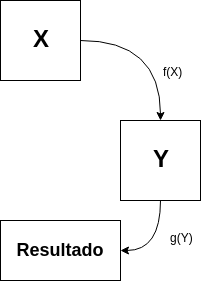
\includegraphics[scale=1]{res/reduccion.png} 
    \caption{Reducciones}
\end{figure}

Este uso de KMP es lejos de ser óptimo, no obtuvimos una complejidad mejor a la fuerza bruta, y en ejecuciones reales los cálculos adicionales de la tabla asistente que hace KMP para lograr un orden lineal realentizan la ejecución suficientemente para que sea un orden entero más lento que una implementación por fuerza bruta. Una mejora sustancial al algoritmo es ejecutar KMP tomando como palabra a ubicar el texto rotado, y como fuente \textbf{una copia duplicada} del texto original, es decir si el texto es \texttt{ABC}, tomaremos como fuente \texttt{ABCABC}. Es fácil de ver que cualquier rotación posible del texto original está completamente contenida dentro de el texto duplicado, tendrá una parte dentro de la primera mitad, y el resto contiguo en la segunda. Con esta estrategia, una única ejecución de KMP es suficiente para poder decidir si un string es rotación de la otra. 

Esta estrategia también es una reducción del problema a uno de string matching resolvible por KMP. Aquí, se debe aplicar una transformación de los datos de entrada para que ``encaje" con el uso que queremos darle a KMP, a diferencia del caso anterior que se pasaban el string original y la potencial rotación como palabra y texto de KMP. El orden mejora sustancialmente al solo ser una única ejecución de KMP, es lineal: la transformación definida también tiene orden lineal, y se hace una única ejecución de la caja negra, a diferencia de la primera versión que hacía N ejecuciones en el peor caso.

Cabe aclarar que las cotas de complejidad temporal que encontramos no son conclusivas, la reducción solo nos puede garantizar que la complejidad del problema que está siendo reducido es, \textit{a lo sumo}, del mismo orden que el algoritmo al que se reduce,asumiendo que las funciones de transformación de datos de entrada y salida son de orden menor o igual a los problemas en sí, que es nuestro caso. El problema de rotaciones cíclicas es entonces, como máximo, de la misma complejidad que el string matching de KMP, pero nada nos dice que no exista una solución que nos de un orden menor. 

\subsubsection{Conclusiones}
El algoritmo por fuerza bruta inicial es un orden cuadrático en la longitud del string. Las reducciones a KMP nos llevan a decir que el problema de rotaciones cícicas es, \textbf{a lo sumo}, de complejidad cuadrática en la primera versión, y lineal en la segunda. No se demuestra que esta última cota es la complejidad real del problema porque la reducción como herramienta no nos permite poder afirmarlo.

A continuación se muestra los tiempos de ejecución de los tres algoritmos para distintos tamaños de cadenas de caracteres. En todos los casos se busca detectar si una cadena de tipo \texttt{AAA...B} es rotación cíclica de \texttt{B...AAA}. De la manera que fueron implementadas las soluciones coincide con el peor caso posible de tiempo de ejecución, en donde se rota N veces la segunda cadena para llegar a la primera. Se puede apreciar los órdenes cuadráticos de las implementaciones por fuerza bruta y KMP no optimizado (ésta mucho más pronunciada que la primera), y la sustancial mejora que se logra cuando se optimiza el código para usar una sola ejecución de KMP.

\begin{table}[h]
    \begin{center}    

    \begin{tabular}{| l | l | l | l |}
        \hline
        longitud (N) & kmp & bruteforce & kmp-optimizado \\ \hline
        1000 & 0.24 & 0.06 & 0.03 \\ \hline
        2000 & 0.82 & 0.15 & 0.03 \\ \hline
        3000 & 1.79 & 0.29 & 0.03 \\ \hline
        4000 & 3.17 & 0.48 & 0.03 \\ \hline
        5000 & 4.94 & 0.75 & 0.03 \\ \hline
        6000 & 7.25 & 1.05 & 0.03 \\ \hline
        7000 & 10.16 & 1.46 & 0.03 \\ \hline
        8000 & 12.96 & 1.85 & 0.03 \\ \hline
        9000 & 16.5 & 2.39 & 0.04 \\ \hline
        10000 & 22.61 & 2.95 & 0.01 \\ \hline
        100000 &  &  & 0.06 \\ \hline
        1000000 &  &  & 0.37 \\ \hline
        5000000 &  &  & 1.74 \\ \hline
    \end{tabular}
    \caption{Tiempos de ejecución en segundos para los distintos algoritmos}
\end{center}
\end{table}

\subsection{Ejercicio 2}
Se demostrará a continuación que el problema es difícil.\\

Se mostrará que \textit{Ciclo Hamiltoniano} $\leq _p$ \textit{TSP}. \\

Dado un grafo dirigido $G=(V,E)$, se define la siguiente instancia del TSP. Se tiene una ciudad $v'_i$ para cada nodo $v_i$ del grafo $G$. Se define $d(v'_i, v'_j)$ igual a 2 de haber una arista $(v_i, v_j)$ en $G$, y se define igual a 1 en caso contrario.\\

$G$ tiene un ciclo Hamiltoniano si y solo si hay un tour de longitud como mínimo $2n$ en el TSP estudiado. Si $G$ tiene un ciclo Hamiltoniano, entonces este ordenamiento de las correspondientes ciudades  define un tour de longitud $2n$. A la inversa, suponga que hay un tour de como mínimo $2n$. La expresión para la longitud de este tour es la suma de $n$ términos, cada uno de los cuales es como máximo $2$, por lo que debe ser el caso que todos los términos son iguales a $2$. Por lo tanto cada par de nodos en $G$ que corresponde a ciudades consecutivas en el tour debe estar conectado por una aristañ se sigue que el ordenamiento de esos correspondientes nodos debe formar un ciclo Hamiltoniano.

\subsection{Ejercicio 3}
Como primer paso, demostraremos que, dada una cantidad $n$ de cursos, si llamamos $m$ a la cantidad máxima de cursos superpuestos en cualquier instante de tiempo, la cantidad de aulas necesarias para realizar la asignación es $m$.\\

\textbf{Demostración}\par
Para demostrar esto, se plantearán las cotas superior e inferior, y se demostrará que ambas coinciden, siendo el valor de ambas: $m$.\\

\textbf{Cota inferior}\par
De haber $m$ cursos que se dictan al mismo tiempo, como no se pueden dictar cursos distintos en una misma aula en simultáneo, queda probado que como mínimo debe haber tantas aulas como cursos se dictan en simultáneo. Por lo tanto, es válido afirmar que $$Aulas\ necesarias \geq m$$\par
\textbf{Cota superior}\par
Para todo instante $t$ de tiempo habrá, según lo demostrado anteriormente, como mínimo $m$ aulas disponibles. Se puede comprobar rápidamente que para ningún $t$ se necesitarán más que $m$ aulas, dado que si dos cursos no se superponen temporalmente, no hay razón por la que no puedan compartir una misma aula. Además se está tratando el caso en que todas las aulas son iguales, lo que evita complicaciones más allá del análisis presentado.

Llegamos entonces a que $$Aulas\ necesarias \leq m$$
Queda así demostrado que $Aulas\ necesarias = m$
\subsubsection{Pseudocódigo}
\begin{algorithm}[H]
    \KwData{Horarios de inicio y finalización de cada uno de los $n$ cursos: $T_{inicio,j}$ y $T_{fin,j}$ denotan los tiempos de inicio y finalización del curso $j-$ésimo. Conjunto de todos los tiempos: $T_i, i\in (1, 2n)$}
    \KwResult{Menor cantidad de aulas necesarias para acomodar todos los cursos suponiendo que todas las aulas son iguales.}
    \BlankLine
    min time slice $\leftarrow \infty$\;
    min time $\leftarrow \infty$\;
    max time $\leftarrow 0$\;
    \ForEach{$T_i$}{
        \If{$(current\ min\ slice = |T_i - T_j|)<min\_aulas, i\neq j$}{
            min time slice := current min\;
        }
        \If{$T_i < $ min time}{
            min time := $T_i$\;
        }
        \If{$T_i > $ max time}{
            max time := $T_i$\;
        }
    }
    \BlankLine
    current time := min time\;
    max superpositions := 0\;
    \While{min time $<$ max time}{
        current num of superpositions := 0\;
        \ForEach{$T_{inicio,j}, T_{fin,j}$}{
            \If{$T_{inicio,j} \geq$ current time slice AND $> T_{fin,j}$}{
                ++current num of superpositions\;
            }
        }
        \If{current num of superpositions $>$ max superpositions}{
            max superpositions := current num of superpositions\;
        }
        current time += min time slice\;
    }
\caption{Pseudo código que resuelve el problema.}
\end{algorithm}
\subsubsection{Reducción a problema de coloreo de grafos}
Considérese cada una de las materias como un nodo. Dados dos nodos, se establece una conexión entre ellos mediante una arista únicamente en caso de superposición horaria entre los cursos que representan dichos nodos. De esta forma, si se encuentra la forma de pintar todos los vértices de forma que no queden dos adyacentes con el mismo color, utilizando la cantidad mínima de colores, se habrá resuelto el problema propuesto.
\subsection{¿P=NP?}
No. 
\end{document}
